\documentclass{article}

% Symbols
\usepackage[T1]{fontenc}
\usepackage{upgreek}
\usepackage{physics}
\usepackage{cancel}
\usepackage{amsfonts, amsthm}
\usepackage{amssymb, latexsym, amsmath}

%Algorithms
\usepackage[ruled,lined,linesnumbered,commentsnumbered]{algorithm2e}

%% Identación
\setlength{\parindent}{0cm}

%% Matrices
\usepackage{amssymb}
\usepackage{amsmath}
\usepackage{amsthm}

% Código
\newcommand{\code}[1]{\textcolor{white!25!black}{\texttt{#1}}}
\usepackage{listings}

%AMS
\usepackage{amsthm}
\newtheorem{algo-thm}{Algoritmo}

% Proof
\renewcommand*{\proofname}{\textbf{Demostraci\'on:}}
% Theorem
\newtheorem*{theorem}{Teorema}

% Graphics
\usepackage{graphicx}
\usepackage{pgf}

% Color a letras.
%\usepackage[usenames,dvipsnames,svgnames,table]{xcolor}

% Tikz
\usepackage{tkz-graph}
\usepackage{tikz}
\usetikzlibrary{arrows,automata}
\usepackage{tikz}
\usetikzlibrary{arrows,automata}
%\usetikzlibrary[topaths]

% Def. Dr. César.
\usetikzlibrary{shapes,calc}
\tikzstyle{edge}=[shorten <=2pt, shorten >=2pt, >=stealth, line width=1.1pt]
\tikzstyle{blueE}=[shorten <=2pt, shorten >=2pt, >=stealth, line width=1.5pt, blue]
\tikzstyle{blackV}=[circle, fill=black, minimum size=6pt, inner sep=0pt, outer sep=0pt]
\tikzstyle{blueV}=[circle, fill=blue, draw, minimum size=6pt, line width=0.75pt, inner sep=0pt, outer sep=0pt]
\tikzstyle{redV}=[circle, fill=red, draw, minimum size=6pt, line width=0.75pt, inner sep=0pt, outer sep=0pt]
\tikzstyle{redSV}=[semicircle, fill=red, minimum size=3pt, inner sep=0pt, outer sep=0pt, rotate=225]
\tikzstyle{blueSV}=[semicircle, fill=blue, minimum size=3pt, inner sep=0pt, outer sep=0pt, rotate=225]
\tikzstyle{blackSV}=[semicircle, fill=black, minimum size=3pt, inner sep=0pt, outer sep=0pt, rotate=225]
\tikzstyle{vertex}=[circle, draw, minimum size=6pt, line width=0.75pt, inner sep=0pt, outer sep=0pt]

% Margins
\addtolength{\voffset}{-1.5cm}
\addtolength{\hoffset}{-1.5cm}
\addtolength{\textwidth}{3cm}
\addtolength{\textheight}{3cm}

%Header-Footer
\usepackage{fancyhdr}
\renewcommand{\headrulewidth}{1pt}

\newcommand{\set}[1]{
  \left\{ #1 \right\}
}

%\pagenumbering{gobble} -- Este comando
%                       -- quita el número de página.
\footskip = 50pt
\renewcommand{\headrulewidth}{1pt}

\pagestyle{fancyplain}

\begin{document}
\title{UNIVERSIDAD NACIONAL AUT\'ONOMA DE M\'EXICO\\ Facultad de Ciencias}
\author{Autor: Adri\'an Aguilera Moreno}
\date{}
\maketitle
\begin{center}
  
\includegraphics[scale=0.20]{../Imagen/Portada.jpg}\\[0.4cm]
  \Large
  \bf{Aut\'omatas y Lenguajes Formales}
  \normalsize
\end{center}
\newpage
\fancyhead[r]{ Aut\'omatas y Lenguajes Formales 2022-2}
%%%%%%%%%%%%%%%%%%%%%%%%%%%%%%%%%%%%%%%%%%%%%%%%%%%%%
\section*{\LARGE{Tarea 2}}
\begin{enumerate}
  %%%%%%%%%%%%%%%%%%%%%% Ejercicio 1.
\item Demuestra que el lenguaje
  \[
  \{\mathbf{a} \in \{a, b, c\}^{*}\; |\; \text{la longitud de $\mathbf{a}$
    es el cuadrado de un natural.}\}
  \]
  no es regular. Usa tanto el teorema del bombeo como el de
  Myhill-Nerode.
  \begin{proof} Antes de iniciar con las demostraciones por los
    teoremas requeridos, analicemos la estructura de las cadenas
    generadas por
    \[
    L(A) = \{\mathbf{a} \in \{a, b, c\}^{*}\; |\; \text{la longitud de $\mathbf{a}$
    es el cuadrado de un natural.}\}
    \]
    Suponiendo que existe el autómata $A \in DFA$ tal que reconoce el lenguaje anterior.
    
    Nótese que $\Sigma = \{a,b,c\}$ y $L(A) = \Sigma^{*}$, entonces $\mathbf{a}$ debe
    ser una cadena finita y supondremos que $L(A)$ es un lenguaje ``muy grande'' pero
    finito.
    
    Además, para nuestras demostraciones nos fijaremos en la longitud de las cadenas
    generadas por nuestro lenguaje y no necesariamente en la estructura de estas
    cadenas, entonces
    \[
    |abababcbacbabc| = |aaaaabbbbbbccc| = |a^{5}b^{6}c^{3}|
    \]
    Lo anterior se puede generalizar usando inducción. Por tanto, en las demostraciones
    supondré, sin pérdida de generalidad, que
    \[
    \mathbf{a} = a^{i}b^{j}c^{r}
    \]
    para $i,j,r \in \mathbb{N}$.
    \begin{center}
      \fbox{
        \begin{minipage}[b][1\height]%
          [t]{0.867\textwidth}
          \textbf{Obs.} El que $\mathbf{a}$ tenga la estructura anterior
          no indica que $b$ siempre debe estar en esa posición, incluso
          podriamos precindir de $b$ o de algún término en la cadena, al
          suponer esa estructura solo simplificamos el considerar casos (que
          por ser un conjunto infinito o muy grande, tendriamos muchas
          combinaciones para concatenar elementos del alfabeto).
      \end{minipage}}
    \end{center}
    Para este ejercicio analicemos $2$ versiones en la
    demostración, \textit{i.e.},
    \newcommand{\localtextbulletone}{\textcolor{black}{\raisebox{.45ex}{\rule{.6ex}{.6ex}}}}
    \renewcommand{\labelitemi}{\localtextbulletone}
    \begin{itemize}
    \item \textbf{Demostración por Teorema del Bombeo.} Procedamos por reducción al absurdo,
      supongamos que el lenguaje dado es regular y que $A = \langle Q_{A}, \Sigma, \delta_{A},
      s, \mathbb{F}_{A} \rangle$ es un autómata determinista finito [en caso de no serlo,
        siempre se puede reducir a un $DFA$] con $k$ estados y $L(A)$ como se definió previamente.
      
      Sea $\mathbf{a} = a^{i}b^{j}c^{r}$ una cadena aceptada por nuestro autómata con
      \[
      i + j + r > k \text{ y al menos } j > k.
      \]
      de lo anterior, podemos deducir que durante la lectura de la cadena $\mathbf{a}$, al
      menos en $2$ ocasiones se pasa por algún estado $q$ en $A$ (es claro que $q$ debe ser
      estado de A). Así, para la función $\delta_{A}$ de transición en $A$, tenemos que
      \begin{eqnarray*}
        \delta^{*}_{A}(s, a^{i}b^{m}) &=& q\\
        \delta^{*}_{A}(q, b^{n}) &=& q\\
        \delta^{*}_{A}(q, b^{l}c^{r}) &=& f \in \mathbb{F}_{A}.
      \end{eqnarray*}
      $\forall_{m,n,l} \in \mathbb{N}$. Donde $m + n + l = j$ y en particular $n \neq 0$ [$b^{n}$
        no se colapsa a $\lambda$].
      
      Como $A$ es determinista, tenemos que para todo $p \in \mathbb{N}$ se cumple que
      \[
      \delta^{*}_{A}(q, b^{np}) = q
      \]
      como consecuencia, directa se tiene que
      \[
      \delta^{*}_{A}(s, a^{i}b^{m}b^{np}b^{l}c^{r}) = f \in \mathbb{F}_{A}.
      \]
      pero $m + np + l \neq j$ cuando $p \neq 1$. Por tanto $ a^{i}b^{m}b^{np}b^{l}c^{r} \in L(A)$,
      lo que implica
      \[
      i + m + np + l + r = t^{2}
      \]
      con $t \in \mathbb{N}$. Sin embargo,
      \[
      i + m + np + l + r = t^{2}\; \not\rightarrow\; i + m + n(p + 1) + l + r = t^{2} + n = x^{2}\; !!!
      \]
      \begin{center}
      \fbox{
        \begin{minipage}[b][1\height]%
          [t]{0.867\textwidth}
          \textbf{Contraejemplo:} Con $i = 6, m = 3, n = 4, l = 2, r = 1$.
          \begin{eqnarray*}
            16 &=& 6 + 3 + 4 + 2 + 1
            \hspace*{4cm} \text{Con } p = 1.\\
            20 &=& 6 + 3 + 4(2) + 2 + 1 = 6 + 3 + 8 + 2 + 1
            \hspace*{0.5cm} \text{Con } p = 2.
          \end{eqnarray*}
          Claramente $20$ no es el cuadrado de un natural.
      \end{minipage}}
    \end{center}      
      lo cual es una contradicción, pues esto debe funcionar para cualquier $p$ natural.
      \[
      \therefore\; \{\mathbf{a} \in \{a, b, c\}^{*}\; |\; \text{la longitud de $\mathbf{a}$
        es el cuadrado de un natural.}\} \text{ \textbf{NO} es regular}.
      \]
    \item \textbf{Demostración por Teorema de Myhill-Nerode.} Por refutación, supongamos que
      $L$ es regular, entonces tenemos que si
      \begin{eqnarray*}
        \alpha &=& (a^{i}b^{j}c^{r})^{w^2}\;\; \text{ tal que } (i + j + r)^{w^2}\;\; = x^{w^2}\; \Rightarrow \alpha \in L.\\
        \beta &=& (a^{m}b^{n}c^{k})^{v^2} \text{ tal que } (m + n + k)^{v^2} = (y)^{v^2} \Rightarrow \beta \in L.\\
        \varphi &=& \alpha.
      \end{eqnarray*}
      Donde $v \neq w$. Así,
      \begin{eqnarray*}
        \alpha \varphi &=& (a^{i}b^{j}c^{r})^{w^2} \cdot (a^{i}b^{j}c^{r})^{w^2}\\
        &=& (a^{i}b^{j}c^{r})^{w^2 + w^2}
        \hspace*{2cm} \text{Aplicando el supuesto del inicio.}\\
        &\Rightarrow& |\alpha \varphi| = (i + j + r)^{w^2 + w^2}\\
        & & \hspace*{0.75cm} = (i + j + r)^{2w^2}\\
        & & \hspace*{0.75cm} = \left((i + j + r)^{w^2}\right)^{2}
      \end{eqnarray*}
      Luego, por el Teorema de Myhill-Nerode tenemos que
      \begin{eqnarray*}
      \alpha \equiv_{L} \beta &\Leftrightarrow& \forall_{n \in \mathbb{N}}\; \alpha \varphi^{n^2} \in L
      \Leftrightarrow \beta \varphi^{n^2} \in L
      \end{eqnarray*}
      Ahora, verifiquemos que $\beta \varphi \in L$, \textit{i.e.},
      \begin{eqnarray*}
        \beta \varphi &=& (a^{m}b^{n}c^{k})^{v^2} \cdot (a^{i}b^{j}c^{r})^{w^2}\\
        &\Rightarrow& (y)^{v^2} \cdot (x)^{w^2} 
      \end{eqnarray*}
      \begin{itemize}
      \item Si $v > w$, entonces
        \begin{eqnarray*}
          y^{v^2 - w^2 + w^2} \cdot x^{w^2} &=& y^{v^2 - w^2} \cdot (xy)^{w^2 + w^2}\\
          &=& y^{v^2 - w^2} \cdot \left((xy)^{w^2}\right)^2 \hspace*{1cm} \text{Se usa el supuesto del principio.}
        \end{eqnarray*}
        sabemos que $v^2 - w^2 = z^2$ solo para $\{v,w,z\}$ una terna pitagórica, y no es
        cierto para cualesquiera naturales, esto contradice que $\beta \varphi \in L$, sin
        embargo nos falta analizar otro caso.
      \item Si $w > v$, entonces
        \begin{eqnarray*}
          y^{w^2 - v^2 + v^2} \cdot x^{w^2} &=& y^{w^2 - v^2} \cdot (xy)^{v^2 + w^2}
        \end{eqnarray*}
        como podemos observar, sucede lo mismo que en el caso anterior, pues
        $w^2 - v^2 = z^2$ y $v^2 + w^2 = t^2$ solo se cumplen para ternas pitagóricas específicas
        y no para cualesquiera naturales.
      \end{itemize}
      De lo anterior, tenemos que $\alpha \not \equiv_{L} \beta$ (pues no hay afinación en $L$),
      lo que implica que existe una cantidad infinita de clases de equivalencias, esto contradice
      el punto $3$ del Teorema de Myhill-Nerode (el tener índice finito), luego
      \[
      \therefore\; \{\mathbf{a} \in \{a, b, c\}^{*}\; |\; \text{la longitud de $\mathbf{a}$
        es el cuadrado de un natural.}\} \text{ \textbf{NO} es regular}.
      \]
    \end{itemize}
    
    En todos los casos se obvia que la demostración para $\mathbf{a} = \lambda$ [cadena vacía] es por vacuidad.
    
    De los analisis anteriores (tanto por Teo. del Bombeo como del Teo. de Myhill-Nerode) concluimos que
    \[
    \therefore\; \{\mathbf{a} \in \{a, b, c\}^{*}\; |\; \text{la longitud de $\mathbf{a}$
      es el cuadrado de un natural.}\} \text{ \textbf{NO} es regular}.
    \]
  \end{proof}
  %%%%%%%%%%%%%%%%%%%%%% Ejercicio 2.
\item Minimiza el autómata de tu respuesta al ejercicio $2$ de la tarea $1$.
  
    $\triangledown$ \textbf{Solución:}
    El autómata del ejercicio $2$ en la tarea $1$ se presenta a continuación:
    \begin{center}
      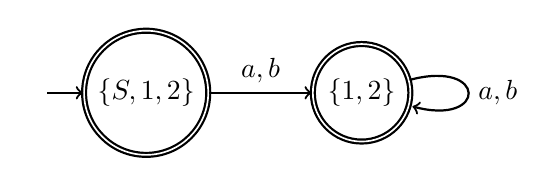
\begin{tikzpicture}[estado/.style={circle,draw=black},auto,/tikz/initial text={},
          final/.style={circle,draw=black,double},thick]
        \node [estado,initial, final] (s12) [left=0pt]  {$\{S,1,2\}$};
        \node [estado,final]           (12) [right=37pt]  {$\{1,2\}$};
        \path[->]
        (s12) edge [curve to, out=0,in=180,relative]  node {$a, b$} (12)
        (12)  edge [loop right]                       node {$a,b$}  (12);
      \end{tikzpicture}
    \end{center}
    Al que llameremos $A$. Para la simplicidad de la solución consideremos
    \begin{eqnarray*}
      \mathbf{S} &=& \{S,1,2\}\\
      \mathbf{q} &=& \{1,2\}
    \end{eqnarray*}
    así, como $\mathbf{S}$ y $\mathbf{q}$ son estados finales, tenemos
    que la matriz que les representa se ve como la que se muestra a
    continuación:
    \[
    \bordermatrix{
                  & \mathbf{S}     & \mathbf{q} \cr
       \mathbf{S} &     n          &      n     \cr
       \mathbf{q} &     n          &      n     \cr
    }
    \]
    \begin{center}
      \fbox{
        \begin{minipage}[b][1\height]%
          [t]{0.867\textwidth}
          \textbf{Obs.} Podemos omitir analizar la diagonal y la parte (triangular)
          inferior de la matriz, pues nuestra matriz es simétrica, y por el algoritmo
          de Minimalización, esto se cumplirá al inicio de las iteraciones y en cuanto
          termine.
      \end{minipage}}
    \end{center}      
    Ahora analicemos la $(2,2)$-pocisión en la matriz con respecto
    al algoritmo de Minimización, esto es
    \begin{eqnarray*}
      (s,q) &=& n.\\
      \left(\delta_A(\mathbf{S}, a), \delta_A(\mathbf{q}, a)\right) &=& (\mathbf{q}, \mathbf{q})\\
      &=& n.\\
      \left(\delta_A(\mathbf{S}, b), \delta_A(\mathbf{q}, b)\right) &=& (\mathbf{q}, \mathbf{q})\\
      &=& n.
    \end{eqnarray*}
    por el algoritmo de Minimalización tenemos que si $(q_{i}, q_{j}) = n$,
    entonces $q_{i} \approx q_{j}$. Por tanto $\mathbf{S} \approx \mathbf{q}$
    [esto es, que formen parte de la misma clase de equivalencia].

    Así, el autómata cociente de $A$ es el que a continuación se presenta:
    \begin{center}
      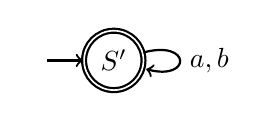
\begin{tikzpicture}[estado/.style={circle,draw=black},auto,/tikz/initial text={},
          final/.style={circle,draw=black,double},thick]
        \node [estado,initial, final] (s) [left=0pt]  {$S'$};
        \path[->]
        (s)  edge [loop right]                       node {$a,b$}  (s);
      \end{tikzpicture}
    \end{center}
    \hfill $\lhd$
    %%%%%%%%%%%%%%%%%%%%%% Ejercicio 3.
  \item Da una CFG para el lenguaje
    \[
    \{a^{n}b^{2n}c^{k}|1 \leq k, n\}.
    \]
    $\triangledown$ \textbf{Solución:}
    
    Sea $G = \langle \{a,b,c\}, \{S, X, Y, Z\}, S, \rightarrow_{G} \rangle$, donde
    las reglas de producción estan dadas por
    \begin{eqnarray*}
      S &\rightarrow_{G}& XYYZ\\
      X &\rightarrow_{G}& a\; |\; aXYY\\
      Y &\rightarrow_{G}& b\\
      Z &\rightarrow_{G}& c\; |\; ZZ
    \end{eqnarray*}
    Para mayor practicidad en los ejercicios siguientes, definimos
    \begin{eqnarray*}
      \Sigma_{G} &=& \{a,b,c\}\\
      \Gamma_{G} &=& \{S,X,Y,Z\}
    \end{eqnarray*}
    de lo anterior, se muestra un ejemplo de derivación con base a la gramática
    propuesta
    \begin{eqnarray*}
      S &\Rightarrow_{G}& XYYZ\\
      &\Rightarrow_{G}& (aXYY)YYZ\\
      &\Rightarrow_{G}& a(a)YYYYZ\\
      &\Rightarrow_{G}& aa(b)YYYZ\\
      &\Rightarrow_{G}& aab(b)YYZ\\
      &\Rightarrow_{G}& aabb(b)YZ\\
      &\Rightarrow_{G}& aabbb(b)Z\\
      &\Rightarrow_{G}& aabbbb(ZZ)\\
      &\Rightarrow_{G}& aabbbb(ZZZ)\\
      &\Rightarrow_{G}& aabbbb(c)ZZ\\
      &\Rightarrow_{G}& aabbbbc(c)Z\\
      &\Rightarrow_{G}& aabbbbcc(c).
    \end{eqnarray*}
    Los paréntesis solo son para ayudar a identificar la sustitución en cada
    iteración.
    \hfill $\lhd$
    %%%%%%%%%%%%%%%%%%%%%% Ejercicio 4.
  \item Transforma la gramática de $3$ a forma normal de Chomsky.
    
    $\triangledown$ \textbf{Solución:}
    Sea $G'$ la gramática a construir. Aplicando la regla 1 del algoritmo de
    transformación a CNF, tenemos que
    \begin{eqnarray*}
      A_{a} &\rightarrow& a\\
      A_{b} &\rightarrow& b\\
      A_{c} &\rightarrow& c
    \end{eqnarray*}
    Así, las reglas de producción se ven modificadas
    \begin{eqnarray*}
      S &\rightarrow& XYYZ\\
      X &\rightarrow& a\; |\; A_aXYY\\
      Y &\rightarrow& b\\
      Z &\rightarrow& c\; |\; ZZ\\
      A_{a} &\rightarrow& a\\
      A_{b} &\rightarrow& b\\
      A_{c} &\rightarrow& c
    \end{eqnarray*}
    Ahora tenemos símbolos no terminales, pero no cumplen ser CNF, los
    únicos que de momento cumplen estar en CNF son los símbolos del alfabeto.
    Luego, por la regla $3$ del algoritmo de transformación a CNF, tenemos que
    \begin{eqnarray*}
      C_{1} &\rightarrow& XY\\
      C_{2} &\rightarrow& YZ\\
      C_{3} &\rightarrow& A_{a}X\\
      C_{4} &\rightarrow& YY
    \end{eqnarray*}
    Ejecutando $4$ y $5$ en el algoritmo de transformación a CNF, obtenemos
    \begin{eqnarray*}
      S &\rightarrow_{G'}& C_{1}C_{2}\\
      X &\rightarrow_{G'}& a\; |\; C_{3}C_{4}\\
      Y &\rightarrow_{G'}& b\\
      Z &\rightarrow_{G'}& c\; |\; ZZ\\
      A_{a} &\rightarrow_{G'}& a\\
      A_{b} &\rightarrow_{G'}& b\\
      A_{c} &\rightarrow_{G'}& c\\
      C_{1} &\rightarrow_{G'}& XY\\
      C_{2} &\rightarrow_{G'}& YZ\\
      C_{3} &\rightarrow_{G'}& A_{a}X\\
      C_{4} &\rightarrow_{G'}& YY
    \end{eqnarray*}
    Eliminando símbolos inútiles tenemos que
    \begin{eqnarray*}
      S &\rightarrow_{G'}& C_{1}C_{2}\\
      X &\rightarrow_{G'}& a\; |\; C_{3}C_{4}\\
      Y &\rightarrow_{G'}& b\\
      Z &\rightarrow_{G'}& c\; |\; ZZ\\
      A_{a} &\rightarrow_{G'}& a\\
      C_{1} &\rightarrow_{G'}& XY\\
      C_{2} &\rightarrow_{G'}& YZ\\
      C_{3} &\rightarrow_{G'}& A_{a}X\\
      C_{4} &\rightarrow_{G'}& YY
    \end{eqnarray*}
    De lo anterior, es claro que $G'$ esta en CNF con:
    \[
    G' = \langle \{a,b,c\}, \{S, C_1, C_2, C_3, X, Y, Z, A_a\}, S, \rightarrow_{G'} \rangle
    \]
    \hfill $\lhd$
    %%%%%%%%%%%%%%%%%%%%%% Ejercicio 5.
  \item Transforma la gramática de $3$ a forma normal de Greibach (basta con
    que presentes algunas reglas de producción representativas).
    
    $\triangledown$ \textbf{Solución:}
    Empecemos encontrando las expresiones regulares (o conjuntos) $R_{A,a}$ que indica la
    iteración $1$ del algoritmo para transformar a GNF, esto es
    \begin{center}
      \fbox{
        \begin{minipage}[b][1\height]%
          [t]{0.867\textwidth}
          Para $R_{S,\alpha}$ con $\alpha \in \Sigma_G$ tenemos que
          \begin{eqnarray*}
            R_{S,a} &=& Y C_2 + X C_4 Y C_2\\
            R_{S,b} = &\{\}& = R_{S,c}
          \end{eqnarray*}
          pues
          \begin{eqnarray*}
            S \Rightarrow C_1 C_2 \Rightarrow X Y C_2 &\Rightarrow& aYC_2.\\
            &\Rightarrow& C_3 C_4 Y C_2 \Rightarrow A_a X C_4 Y C_2  \Rightarrow a X C_4 Y C_2.
          \end{eqnarray*}
      \end{minipage}}
    \end{center}
    
    \begin{center}
      \fbox{
        \begin{minipage}[b][1\height]%
          [t]{0.867\textwidth}
          Para $R_{X,\alpha}$ con $\alpha \in \Sigma_G$ tenemos que
          \begin{eqnarray*}
            R_{X,a} &=& \lambda + X C_4 \\
            R_{X,b} = &\{\}& = R_{X,c}
          \end{eqnarray*}
          pues
          \begin{eqnarray*}
            X \Rightarrow C_3 C_4 \Rightarrow  A_a X C_4  \Rightarrow a X C_4 .
          \end{eqnarray*}
      \end{minipage}}
    \end{center}
    
    \begin{center}
      \fbox{
        \begin{minipage}[b][1\height]%
          [t]{0.867\textwidth}
          Para $R_{Y,\alpha}$ con $\alpha \in \Sigma_G$ tenemos que
          \begin{eqnarray*}
            R_{Y,b} &=& \lambda \\
            R_{Y,a} = &\{\}& = R_{Y,c}
          \end{eqnarray*}
          pues $Y \Rightarrow b$.
      \end{minipage}}
    \end{center}
    
    \begin{center}
      \fbox{
        \begin{minipage}[b][1\height]%
          [t]{0.867\textwidth}
          Para $R_{Z,\alpha}$ con $\alpha \in \Sigma_G$ tenemos que
          \begin{eqnarray*}
            R_{Z,c} &=& \lambda + Z\\
            R_{Z,a} = &\{\}& = R_{Z,b}
          \end{eqnarray*}
          pues
           \begin{eqnarray*}
            Z &\Rightarrow& C.\\
            &\Rightarrow& ZZ \Rightarrow cZ.
           \end{eqnarray*}
           en este caso en particular podemos producir $Z \Rightarrow Z \dotsm Z$
           un número a lo más de $k$ veces, sin embargo nuestra definición de $Z$
           es suficiente\footnote{pues $k$ es un natural, por tanto la cadena $Z
           \Rightarrow Z \dotsm Z$ es finita.} y es por esto que no se incluyen
           en la expresión regular de $R_{Z,c}$.
      \end{minipage}}
    \end{center}
    
    \begin{center}
      \fbox{
        \begin{minipage}[b][1\height]%
          [t]{0.867\textwidth}
          Para $R_{C_1,\alpha}$ con $\alpha \in \Sigma_G$ tenemos que
          \begin{eqnarray*}
            R_{C_1,a} &=& Y + X C_4 Y\\
            R_{C_1,b} = &\{\}& = R_{C_1,c}
          \end{eqnarray*}
          pues
          \begin{eqnarray*}
            C_1 \Rightarrow XY &\Rightarrow& aY.\\
            &\Rightarrow& C_3 C_4 Y \Rightarrow A_a X C_4 Y \Rightarrow a X C_4 Y.
          \end{eqnarray*}
      \end{minipage}}
    \end{center}
    
    \begin{center}
      \fbox{
        \begin{minipage}[b][1\height]%
          [t]{0.867\textwidth}
          Para $R_{C_2,\alpha}$ con $\alpha \in \Sigma_G$ tenemos que
          \begin{eqnarray*}
            R_{C_2,b} &=& Z \\
            R_{C_2,a} = &\{\}& = R_{C_2,c}
          \end{eqnarray*}
          pues $C_2 \Rightarrow YZ \Rightarrow bZ$.
      \end{minipage}}
    \end{center}
    
    \begin{center}
      \fbox{
        \begin{minipage}[b][1\height]%
          [t]{0.867\textwidth}
          Para $R_{C_3,\alpha}$ con $\alpha \in \Sigma_G$ tenemos que
          \begin{eqnarray*}
            R_{C_3,a} &=& X \\
            R_{C_3,b} = &\{\}& = R_{C_3,c}
          \end{eqnarray*}
          pues $C_3 \Rightarrow A_a X \Rightarrow aX$.
      \end{minipage}}
    \end{center}
    
    \begin{center}
      \fbox{
        \begin{minipage}[b][1\height]%
          [t]{0.867\textwidth}
          Para $R_{C_4,\alpha}$ con $\alpha \in \Sigma_G$ tenemos que
          \begin{eqnarray*}
            R_{C_4,a} &=& X \\
            R_{C_4,b} = &\{\}& = R_{C_4,c}
          \end{eqnarray*}
          pues $C_4 \Rightarrow Y Y \Rightarrow bY$.
      \end{minipage}}
    \end{center}
    Ahora, encontremos las gramáticas lineales por la izquierda que indica
    la iteración $2$ del algoritmo de transformación a GNF, esto es
    \begin{eqnarray*}
      T_{S,a} &\rightarrow& Y C_2\; |\; X C_4 Y C_2\\
      T_{X,a} &\rightarrow& \lambda\; |\; X C_4\;\\
      T_{Y,b} &\rightarrow& \lambda\\
      T_{Z,c} &\rightarrow& \lambda\; |\; Z\\
      T_{C_1,a} &\rightarrow& Y\; |\; X C_4 Y\\
      T_{C_2,b} &\rightarrow& Z\\
      T_{C_3,a} &\rightarrow& X\\
      T_{C_4,a} &\rightarrow& Y
    \end{eqnarray*}
    Bajo la misma iteración, sustituimos las reglas para llevarlas a la forma
    GNF
    \begin{eqnarray*}
      Y &\rightarrow& b\\
      A_a &\rightarrow& a\\
      S &\rightarrow& a T_{C_1, a} C_2
      \hspace*{2cm} \text{Sustituimos en } S \text{ de } G'.\\
      X &\rightarrow& a\; |\; a T_{C_3, a} C_4
      \hspace*{1.5cm} \text{Sustituimos en } X \text{ de } G'.\\
      Z &\rightarrow& c\; |\; c Z
      \hspace*{2.5cm} \text{Sustituimos en } Z \text{ de } G'.\\
      C_1 &\rightarrow& aY\; |\; a X C_4 Y
      \hspace*{1.4cm} \text{Sustituimos en } C_1 \text{ de } G'.\\
      C_2 &\rightarrow& bZ
      \hspace*{2.9cm} \text{Sustituimos en } C_2 \text{ de } G'.\\
      C_3 &\rightarrow& aX
      \hspace*{2.8cm} \text{Sustituimos en } C_3 \text{ de } G'.\\
      C_4 &\rightarrow& bY
      \hspace*{2.9cm} \text{Sustituimos en } C_4 \text{ de } G'.\\
      T_{S,a} &\rightarrow& b C_2\; |\; a C_4 Y C_2\; |\; a T_{c_3, a} C_4 Y C_2\\
      T_{X,a} &\rightarrow& \lambda\; |\; a C_4\; |\; a T_{C_3, a} C_4^2\\
      T_{Y,b} &\rightarrow& \lambda\\
      T_{Z,c} &\rightarrow& \lambda\; |\; bZ\\
      T_{C_1,a} &\rightarrow& b\; |\; a C_4 Y\; |\; a T_{C_3,a} C_4^2 Y\\
      T_{C_2,b} &\rightarrow& c|cZ\\
      T_{C_3,a} &\rightarrow& a\; |\; a T_{C_3, a} C_4\\
      T_{C_4,a} &\rightarrow& b
    \end{eqnarray*}
    Para todas las $T_{i,j}$ se hacen modificaciones con respecto a la gramática lineal
    generada con anterioridad.
    
    Ahora, por la iteración $3$ del algoritmo de transformación a GNF, procedamos a
    eliminar las producciones-$\varepsilon$. Así,
    \begin{eqnarray*}
      Y &\rightarrow& b\\
      A_a &\rightarrow& a\\
      S &\rightarrow& a T_{C_1, a} C_2\\
      X &\rightarrow& a\; |\; a T_{C_3, a} C_4 \\
      Z &\rightarrow& c\; |\; c Z\\
      C_1 &\rightarrow& aY\; |\; a X C_4 Y\\
      C_2 &\rightarrow& bZ\\
      C_3 &\rightarrow& aX\\
      C_4 &\rightarrow& bY\\
      T_{S,a} &\rightarrow& b C_2\; |\; a C_4 Y C_2\; |\; a T_{c_3, a} C_4 Y C_2\\
      T_{X,a} &\rightarrow&  a C_4\; |\; a T_{C_3, a} C_4^2\\
      %T_{Y,b} &\rightarrow& \lambda\\
      T_{Z,c} &\rightarrow&  bZ\\
      T_{C_1,a} &\rightarrow& b\; |\; a C_4 Y\; |\; a T_{C_3,a} C_4^2 Y\\
      T_{C_2,b} &\rightarrow& c|cZ\\
      T_{C_3,a} &\rightarrow& a\; |\; a T_{C_3, a} C_4\\
      T_{C_4,a} &\rightarrow& b
    \end{eqnarray*}
    por último eliminemos los símbolos inaccesibles, \textit{i.e.},
    \begin{eqnarray*}
      S &\rightarrow& a T_{C_1, a} C_2\\
      Y &\rightarrow& b\\
      A_a &\rightarrow& a\\
      X &\rightarrow& a\; |\; a T_{C_3, a} C_4 \\
      Z &\rightarrow& c\; |\; c Z\\
      %C_1 &\rightarrow& aY\; |\; a X C_4 Y\\
      C_2 &\rightarrow& bZ\\
      %C_3 &\rightarrow& aX\\
      C_4 &\rightarrow& bY\\
      %T_{S,a} &\rightarrow& b C_2\; |\; a C_4 Y C_2\; |\; a T_{c_3, a} C_4 Y C_2\\
      %T_{X,a} &\rightarrow&  a C_4\; |\; a T_{C_3, a} C_4^2\\
      %T_{Y,b} &\rightarrow& \lambda\\
      %T_{Z,c} &\rightarrow&  bZ\\
      %T_{C_1,a} &\rightarrow& b\; |\; a C_4 Y\; |\; a T_{C_3,a} C_4^2 Y\\
      T_{C_2,b} &\rightarrow& c|cZ\\
      T_{C_3,a} &\rightarrow& a\; |\; a T_{C_3, a} C_4
      %T_{C_4,a} &\rightarrow& b
    \end{eqnarray*}
    Se puede comprobar por fuerza bruta (y por inducción) que la gramática
    anterior se encuentra en GNF.
    \hfill $\lhd$
  \item Demuestra que el conjunto
    \[
    \{a^n b^m c^k\; |\; n = k \land k = 3m\}
    \]
    no es un CFL.
    \begin{proof}
      Veamos que nuestro lenguaje es equivalente a
      \[
       \{a^{3m} b^m c^{3m}\}
      \]
      Así, analicemos $6$ posibles casos:
      \newcommand{\localtextbulletone}{\textcolor{black}{\raisebox{.45ex}{\rule{.6ex}{.6ex}}}}
      \renewcommand{\labelitemi}{\localtextbulletone}
      \begin{itemize}
      \item Supongamos, sin pérdida de generalidad, que bombearemos $a^i$ [un extremo\footnote{Nótese que esto es análogo a bombear $c^i$.}]
        en nuestro lenguaje. Esto es,
        \begin{eqnarray*}
          a^{3m - i} \underbrace{a \dotsm a}_{\alpha} b^m c^{3m}
        \end{eqnarray*}
        
        \begin{center}
          \fbox{
            \begin{minipage}[b][1\height]%
              [t]{0.867\textwidth}
              \textbf{Obs.} Se puede bombear en cualquier parte de la cadena de $a$'s.
          \end{minipage}}
        \end{center}

        con $|\alpha| = ri \in \mathbb{N}$. Esto se cumple solo cuando $r = 1$, en otro caso
        \begin{itemize}
        \item $r > 1$. Entonces,
          \begin{eqnarray*}
            (3m - i) + i &<& (3m - i) + ri\\
            \Rightarrow 3m &<& (3m - i) + ri.
          \end{eqnarray*}
          lo que implica que $|a^{3m - i}\alpha| > |c^{3m}|$, ahora es claro que esa cadena no esta en $L$.
        \item $r = 0$. Entonces,
          \begin{eqnarray*}
            (3m - i) + i &>& (3m - i) + ri\\
            &>& (3m - i) + 0\\
            \Rightarrow 3m &>& 3m - i.
          \end{eqnarray*}
          lo que implica que $|a^{3m - i}\alpha| < |c^{3m}|$, ahora es claro que esa cadena no esta en $L$.
        \end{itemize}
        
      \item  Supongamos, sin pérdida de generalidad, que bombearemos $a^i$ y $c^j$ [Extremos]
        en nuestro lenguaje. Esto es,
        \begin{eqnarray*}
          a^{3m - i} \underbrace{a \dotsm a}_{\alpha} b^m \underbrace{c \dotsm c}_{\varphi}c^{3m - j}
        \end{eqnarray*}
        
        \begin{center}
          \fbox{
            \begin{minipage}[b][1\height]%
              [t]{0.867\textwidth}
              \textbf{Obs.} Se puede bombear en cualquier parte de las cadenas de $a$'s y $c$'s respectivamente.
          \end{minipage}}
        \end{center}
        
        con
        \begin{itemize}
        \item $|\alpha| = ri = rj = |\beta| \neq 1$. Entonces,
          
          Caso 1: $ri = 0$.
          \begin{eqnarray*}
            3m &>& (3m - i) + ri = (3m - j) + pj\\
            &>& 3m - i = 3m - j.
          \end{eqnarray*}
          lo que implica que $3|b^m| > |a^{3m - i}\alpha| = |c^{3m - j}\beta|$, ahora es claro que esa cadena no esta en $L$.
          
          Caso 2: $ri > 1$.
          \begin{eqnarray*}
            3m &<& (3m - i) + ri = (3m - j) + pj\\
            &<& 3m + (r - 1)i = 3m + (p - 1)j.
          \end{eqnarray*}
          el caso mínimo es cuando $r = 2 = p$, entonces nos quedan $3m + i = 3m + j$ como longitudes de $\alpha$
          y $\beta$ respectivamente, luego descartamos la cadena de $L$ por no cumplir que $ |a^{3m - i}\alpha| = 3|b^m| = |c^{3m - j}\beta|$.
        \item $|\alpha| \neq |\beta|$ y $|\alpha| = ri$, $|\beta| = pj$. Entonces,
          \begin{eqnarray*}
            3m \neq (3m - i) + ri &\text{ y }& 3m \neq (3m - j) + pj\\
            \hspace{0.5cm} \neq 3m + (r - 1)i. & & \hspace*{0.6cm}\neq 3m + (p - 1)j.
          \end{eqnarray*}
          lo cual es claro por los ejemplos más desarrollados arriba. Así, esas cadenas no pertenecen
          a $L$.
        \end{itemize}
      \item Supongamos, sin pérdida de generalidad, que bombearemos $b^i$ [Medio]
        en nuestro lenguaje. Esto es,
        
        \begin{eqnarray*}
          a^{3m} b^{m- (i + j)}\underbrace{b \dotsm b}_{\alpha} b^{j} c^{3m}
        \end{eqnarray*}
        
        \begin{center}
          \fbox{
            \begin{minipage}[b][1\height]%
              [t]{0.867\textwidth}
              \textbf{Obs.} Se puede bombear en cualquier parte de la cadena de $b$'s.
          \end{minipage}}
        \end{center}
        
        con $|\alpha| = ri$. Entonces la cadena solo pertenece a $L$ cuando $r = 1$, en otro caso
        \[
        m - (i + j) + i + j = m \not= m - (i + j) + ri + j
        \]
        Así, las cadenas de esa forma no son parte de $L$.
      \item Supongamos, sin pérdida de generalidad, que bombearemos las subcadenas $a^{i}$ y $b^{j}$
        [Medio y un extremo \footnote{Esto es análogo a bombear $b^{i}$ y $c^{j}$.}] en nuestro lenguaje.
        Esto es,
        \begin{eqnarray*}
          a^{3m - i} \underbrace{a \dotsm a}_{\alpha} b^{m- j}\underbrace{b \dotsm b}_{\beta} c^{3m}
        \end{eqnarray*}
        
        \begin{center}
          \fbox{
            \begin{minipage}[b][1\height]%
              [t]{0.867\textwidth}
              \textbf{Obs.} Se puede bombear en cualquier parte de las cadenas de $a$'s y $b$'s respectivamente.
          \end{minipage}}
        \end{center}
        
        con $|\alpha| = ri$ y $|\beta| = pj$. De lo anterior, la única cadena que esta en el lenguaje es cuando
        $r = 1 = p$. En otro caso, pasa el primer caso y el anterior, con lo cual ya vimos que las cadenas generadas
        no pertenecen a $L$.
      \item Otro caso que vale la pena analizar y es más obvio de notar (que no pertenece a $L$), es cuando se bombea
        $a^i b^j$, pues el único caso que es aceptado por $L$ es cuando se bombea una solo vez, en otro caso tendriamos
        algo como lo siguiente
        \[
        a^{3m - i} a^i b^j \dotsm a^i b^j b^{m - j} c^{3m} 
        \]
        o como lo siguiente
       \[
        a^{3m - i} b^{m - j} c^{3m} 
        \]
        y como $|a^{3m - i}| < |c^{3m}|$ (o por el caso $1$), deducimos que no pertenece a $L$.
      \item Un último caso a analizar (y que también es fácil de ver, el porque no pertenece a $L$)
        es cuando se bombea $a^i b^m c^j$, pues se tendría que cuando se bombea una cantidad de
        veces distinta de $1$ se tiene que
        \begin{eqnarray*}
          a^{3m - i} a^i b^m c^j \dotsm  a^i b^m c^j  c^{3m - j}.
        \end{eqnarray*}
      \end{itemize}
      Después del análisis anterior, podemos concluir que $L \notin$ CFL.
    \end{proof}
\end{enumerate}
\end{document}
